\section{Results}
\label{sec:results}

\subsection{Main Results}

Table~\ref{tab:main_results} reports mean F1, precision, recall, and perfect-score
count across all 200 patients for each model--strategy combination. Two results stand out immediately. Performance varies enormously, from F1 = 0.0000 for
BioMistral on all four strategies, to F1 = 0.9956 for Llama-3.3-70B on Strategy A.
And which strategy performs best depends on model size, a finding we show is
statistically significant.

\begin{table*}[t]
\centering
\small
\resizebox{\textwidth}{!}{%
\begin{tabular}{llrrrrrrr}
\toprule
\textbf{Model} & \textbf{Strategy} & \textbf{Mean F1} & \textbf{Mean Prec.} & \textbf{Mean Rec.} & \textbf{Median F1} & \textbf{Perfect} & \textbf{Zero F1} & \textbf{Parse Fail} \\
\midrule
Phi-3.5-mini (3.8B) & A & 0.6356 & 0.7296 & 0.5932 & 0.7596 & 75  & 45  & 33 \\
Phi-3.5-mini (3.8B) & B & 0.6833 & 0.8111 & 0.6264 & 0.7500 & 64  & 25  & 16 \\
Phi-3.5-mini (3.8B) & C & \textbf{0.7008} & 0.7616 & 0.6670 & 0.8000 & 66  & 28  &  7 \\
Phi-3.5-mini (3.8B) & D & 0.6443 & 0.7703 & 0.5902 & 0.6905 & 61  & 30  & 11 \\
\midrule
Mistral-7B          & A & 0.7247 & 0.8886 & 0.6684 & 0.8889 & 87  & 20  & 11 \\
Mistral-7B          & B & 0.8753 & 0.9646 & 0.8344 & 1.0000 & 122 &  6  &  3 \\
Mistral-7B          & C & \textbf{0.9149} & 0.9319 & 0.9026 & 1.0000 & 153 & 10  &  5 \\
Mistral-7B          & D & 0.8588 & 0.9611 & 0.8100 & 1.0000 & 112 &  6  &  3 \\
\midrule
BioMistral-7B       & A & 0.0000 & 0.0000 & 0.0000 & 0.0000 &  0  & 200 & 198 \\
BioMistral-7B       & B & 0.0000 & 0.0000 & 0.0000 & 0.0000 &  0  & 200 & 197 \\
BioMistral-7B       & C & 0.0000 & 0.0000 & 0.0000 & 0.0000 &  0  & 200 & 198 \\
BioMistral-7B       & D & 0.0000 & 0.0000 & 0.0000 & 0.0000 &  0  & 200 & 198 \\
\midrule
Llama-3.1-8B        & A & 0.9180 & 0.9629 & 0.9052 & 1.0000 & 138 &  2  &  0 \\
Llama-3.1-8B        & B & 0.9250 & 0.9562 & 0.9182 & 1.0000 & 147 &  1  &  0 \\
Llama-3.1-8B        & C & \textbf{0.9471} & 0.9513 & 0.9448 & 1.0000 & 173 &  5  &  2 \\
Llama-3.1-8B        & D & 0.9228 & 0.9724 & 0.8995 & 1.0000 & 144 &  2  &  1 \\
\midrule
Llama-3.3-70B       & A & \textbf{0.9956} & 1.0000 & 0.9929 & 1.0000 & 196 &  0  &  0 \\
Llama-3.3-70B       & B & 0.9867 & 0.9900 & 0.9845 & 1.0000 & 194 &  2  &  2 \\
Llama-3.3-70B       & C & 0.9850 & 0.9850 & 0.9850 & 1.0000 & 197 &  3  &  3 \\
Llama-3.3-70B       & D & 0.8742 & 0.8750 & 0.8736 & 1.0000 & 174 & 25  &  2 \\
\bottomrule
\end{tabular}%
}
\caption{Aggregate results across all 200 patients ($n = 200$) per model and strategy.
  Strategy labels: A = Raw JSON, B = Markdown Table, C = Clinical Narrative,
  D = Chronological Timeline (full definitions in Section~\ref{sec:strategies}).
  Best strategy per model (excluding BioMistral) is in bold. Strategy C is best for
  all instruction-tuned models up to 8B; Strategy A becomes best at 70B.}
\label{tab:main_results}
\end{table*}

\subsection{The Serialisation Strategy Effect}
\label{sec:strategy_effect}

Figure~\ref{fig:heatmap} shows F1 by model and strategy as a heatmap.
For instruction-tuned models up to 8B parameters, Strategy C (Clinical Narrative)
achieves the highest mean F1 for all instruction-tuned models up to 8B: 0.7008 for Phi-3.5-mini (vs.\ 0.6356
with Strategy A), 0.9149 for Mistral-7B (vs.\ 0.7247), and 0.9471 for Llama-3.1-8B
(vs.\ 0.9180). At 70B parameters, the ranking reverses: Strategy A achieves F1 =
0.9956, which is slightly but meaningfully higher than Strategy C (0.9850). Strategy
D performs poorly at 70B (F1 = 0.8742 with 25 zero-F1 patients), suggesting that
temporal reasoning under this format is surprisingly difficult even for the largest model.

\begin{figure}[t]
  \centering
  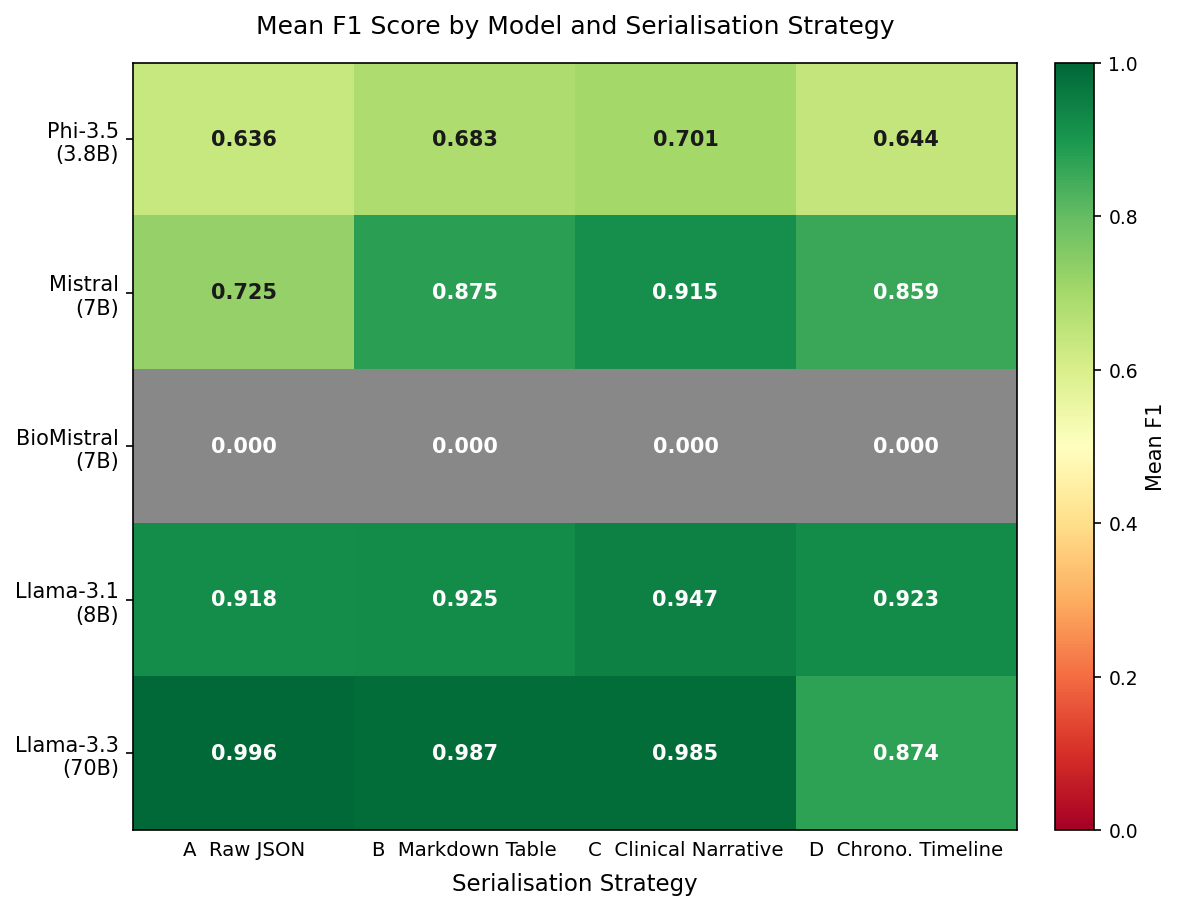
\includegraphics[width=\columnwidth]{figures/01_heatmap_f1.png}
  \caption{Mean F1 by model and serialisation strategy. Each cell shows the mean F1
           across 200 patients. Strategy C is best for $\leq$8B models; Strategy A
           is best at 70B.}
  \label{fig:heatmap}
\end{figure}

\begin{figure}[t]
  \centering
  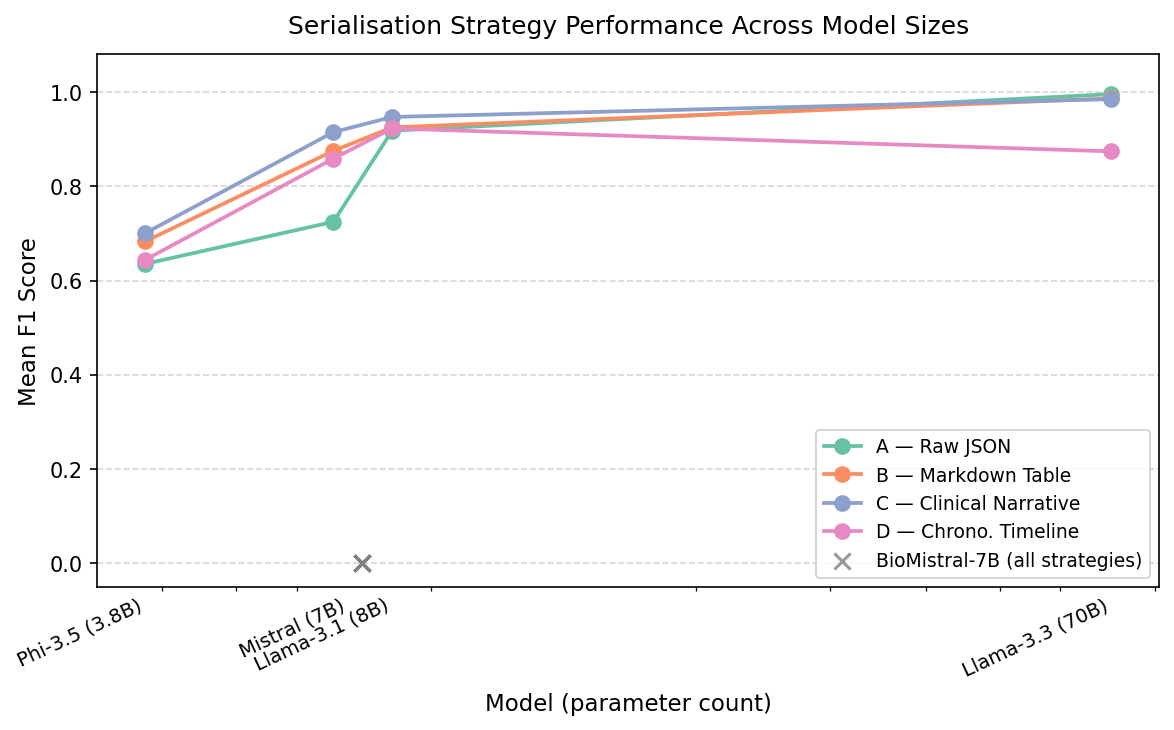
\includegraphics[width=\columnwidth]{figures/03_strategy_rank_by_size.png}
  \caption{Mean F1 per strategy across model sizes (x-axis on log scale).
           The strategy ranking inverts between 8B and 70B.}
  \label{fig:strategy_rank}
\end{figure}

Statistical tests confirm these observations (Table~\ref{tab:stats}). For Mistral-7B,
the advantage of Strategy C over Strategy A is large and highly significant
($r = 0.617$, $p < 10^{-10}$, Bonferroni-corrected). For Llama-3.1-8B the effect is
medium ($r = 0.345$, $p = 0.011$). For Phi-3.5-mini and Llama-3.3-70B, no significant
difference is found after correction. Phi-3.5-mini is near its performance ceiling on
this task, and Llama-3.3-70B performs near-perfectly under all formats.

\begin{table}[h]
\centering
\small
\resizebox{\columnwidth}{!}{%
\begin{tabular}{llrrrl}
\toprule
\textbf{Model} & \textbf{Test} & $W$ & $p$ (corr.) & $r$ & \\
\midrule
Phi-3.5-mini   & A vs C & 3143 & 0.106  & 0.197 & ns \\
Mistral-7B     & A vs C &  948 & $< 10^{-10}$ & 0.617 & *** \\
Llama-3.1-8B   & A vs C &  859 & 0.011  & 0.345 & * \\
Llama-3.3-70B  & A vs C &   10 & 1.000  & 0.257 & ns \\
\midrule
\multicolumn{6}{l}{\textit{Cross-model comparisons on Strategy C}} \\
Mistral vs Llama-3.1-8B       & --- & 414 & 0.019       & 0.327 & *   \\
Llama-3.1-8B vs Llama-3.3-70B & --- &  22 & $< 10^{-3}$ & 0.757 & *** \\
\bottomrule
\end{tabular}%
}
\caption{Wilcoxon signed-rank tests. A vs C: Bonferroni-corrected ($k=4$).
  Significance: *** $p < 0.001$, * $p < 0.05$, ns not significant.
  $r = |Z| / \sqrt{N}$.}
\label{tab:stats}
\end{table}

\subsection{Omission Dominates Hallucination}
\label{sec:omission}

Figure~\ref{fig:scatter} shows precision versus recall for each model--strategy
combination. In all 20 model and strategy combinations, mean precision is equal to or
higher than mean recall. Omission is the dominant failure mode: models return a subset
of the true active medication list more often than they fabricate spurious entries.
Hallucinations do occur — precision falls as low as 0.73 for Phi-3.5-mini on Raw JSON
— but at lower rates than omissions in every setting we tested.

\begin{figure}[t]
  \centering
  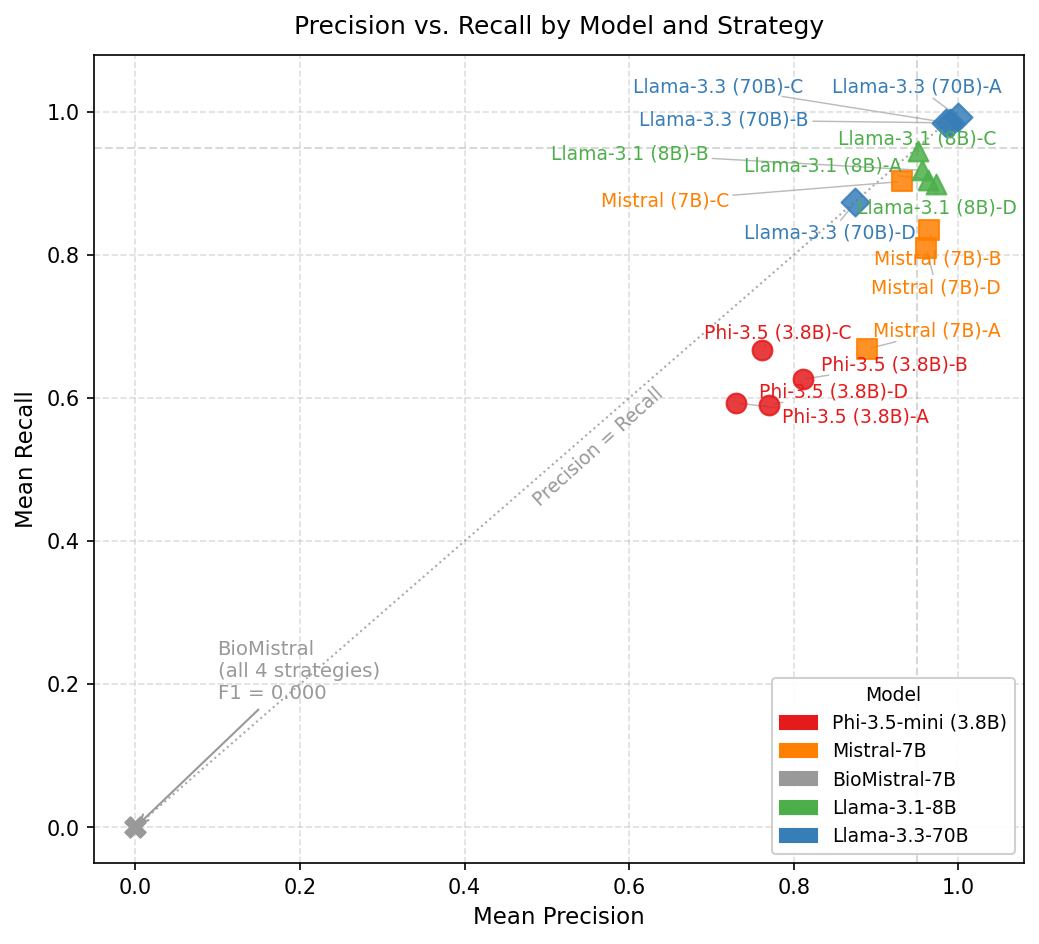
\includegraphics[width=\columnwidth]{figures/06_precision_recall_scatter.png}
  \caption{Precision vs.\ recall for each (model, strategy) pair. All points lie
           on or above the diagonal: omission rates exceed hallucination rates in
           every model--strategy combination.}
  \label{fig:scatter}
\end{figure}

This has direct clinical implications. The asymmetry means model output is a
\textit{partial} but \textit{higher-confidence} list of active medications. Clinicians
reviewing the output face a completeness-checking task — what did the model miss? —
rather than an equally heavy accuracy-checking task against both false positives and
false negatives.

\paragraph{What gets omitted.}
Aggregating false-negative medication names across all 200 patients reveals a clear
length bias. Omitted medications are systematically longer than retained ones: for
Mistral-7B on Clinical Narrative, 37\% of the 114 omissions have names exceeding 50
characters against a 22\% baseline among true positives; for Phi-3.5-mini on the same
strategy the gap widens to 43\% vs.\ 14\%; for Llama-3.3-70B on the Chronological
Timeline, 41\% vs.\ 22\% of 102 omissions. The most-missed single medication across
smaller models is \textit{Hydrochlorothiazide 25 MG Oral Tablet}, a first-line
antihypertensive (missed by Mistral-7B on Strategy A in 34 of 53 patients where it is
active). Top-5 omissions across models are dominated by common cardiovascular agents
(lisinopril, metoprolol succinate, simvastatin, clopidogrel), which are disproportionately
represented in the cohort and prescribed chronically with many refill entries. A
portion of Llama-3.3-70B's Strategy D precision errors are formatting variants of
correct active medications — for example \textit{lisinopril 10 MG Oral Tablet (RxNorm:
314076)} against a ground truth string without the RxNorm suffix — which under exact
matching count as both a false positive and a false negative, reinforcing that the
reported precision values are conservative lower bounds.

\subsection{Capacity Ceiling for Complex Patients}
\label{sec:ceiling}

Figure~\ref{fig:recall_gt} shows mean recall binned by the number of active
medications in the ground truth. For models up to 8B parameters, performance degrades
sharply with increasing medication count. Mistral-7B recall falls from 0.96 for
patients with a single active medication to 0.24 for patients with 11 active
medications. Llama-3.1-8B degrades more gracefully but still drops from near-perfect
at 1--2 medications to roughly 0.80 at 10+. Llama-3.3-70B holds near-perfect recall
through 16 active medications with virtually no degradation.

\begin{figure}[t]
  \centering
  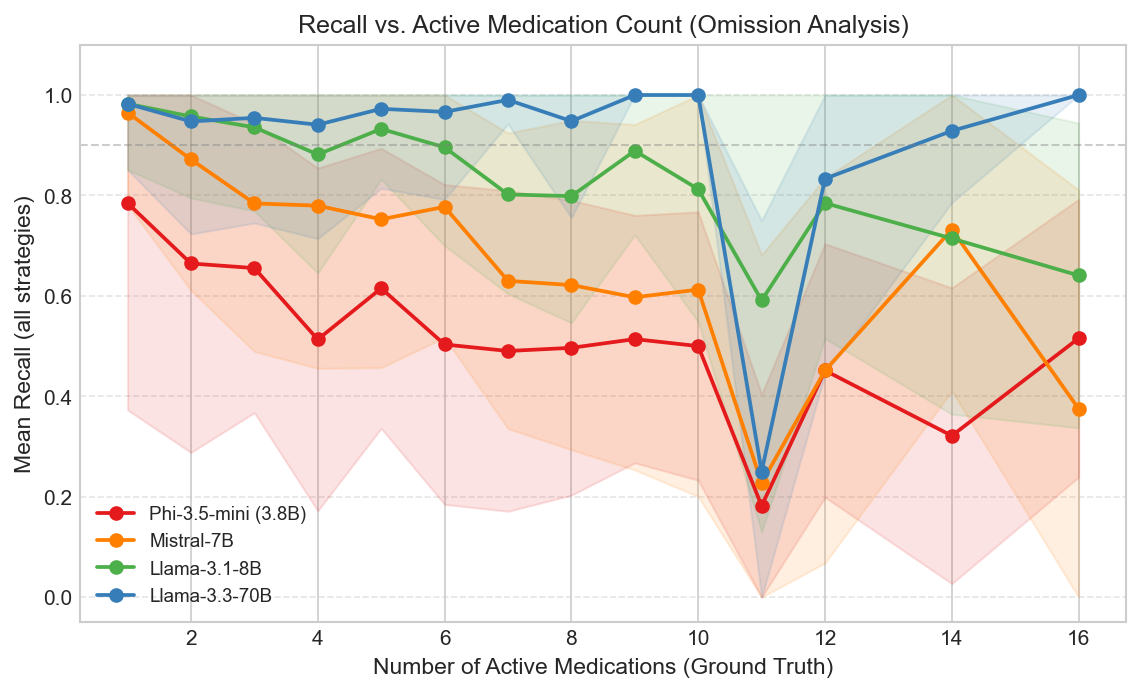
\includegraphics[width=\columnwidth]{figures/04_recall_vs_gt_count.png}
  \caption{Mean recall by number of active medications in the ground truth. Smaller
           models plateau sharply around 7--10 active medications; Llama-3.3-70B
           remains near-perfect.}
  \label{fig:recall_gt}
\end{figure}

Crucially, history length (total years of medication records) does not predict
failure. Figure~\ref{fig:recall_span} confirms this: mean recall is flat across
history spans from 10 to 25+ years for every model. Only the number of
\textit{currently active} medications degrades recall. The bottleneck is output
generation capacity---listing all active medications in one response---not
input processing or reasoning over a long record.

\begin{figure}[t]
  \centering
  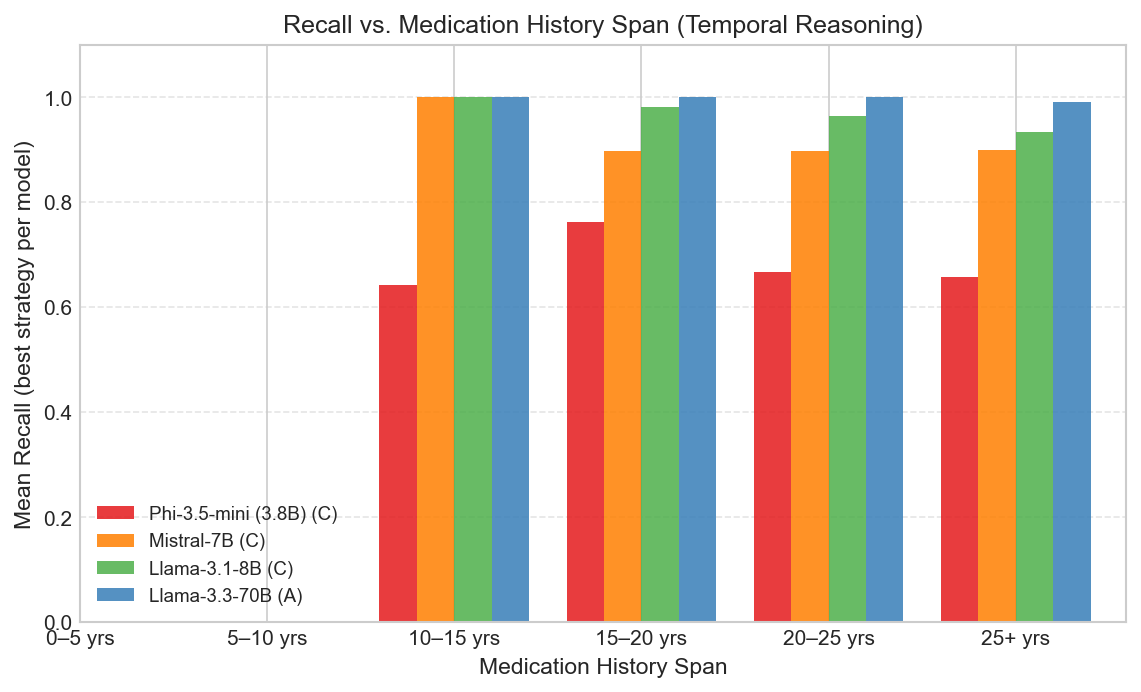
\includegraphics[width=\columnwidth]{figures/05_recall_vs_history_span.png}
  \caption{Mean recall by total medication history span (best strategy per model).
           Recall is flat across all history lengths, with no degradation as records
           grow longer. History span does not predict failure; only the count of
           currently active medications does (Figure~\ref{fig:recall_gt}).}
  \label{fig:recall_span}
\end{figure}

\subsection{BioMistral: Instruction Following Failure}
\label{sec:biomistral}

BioMistral-7B achieves F1 = 0.0000 on all 200 patients across all four strategies.
Its sibling model, Mistral-7B v0.1 (same architecture, same parameter count), achieves
F1 = 0.9149 on Strategy C. The difference is not due to domain knowledge: BioMistral
was further-pretrained on PubMed Central text \textit{starting from} Mistral-7B
Instruct v0.1, which should have preserved its instruction-following capabilities in
principle.

Inspection of raw outputs reveals two failure modes, shown in
Figure~\ref{fig:bio_failures}: (1) garbled or incoherent token sequences
(113--140 patients depending on strategy) and (2) the model continuing the
system prompt verbatim rather than generating a response (11--68 patients).
A small number of runs produced an empty response or a generic chatbot greeting.
In no case did BioMistral return a parseable JSON array. The catastrophic
forgetting of instruction-following behaviour during domain-continued pretraining
renders the model entirely unusable for structured extraction tasks, regardless
of the input format.

\begin{figure}[t]
  \centering
  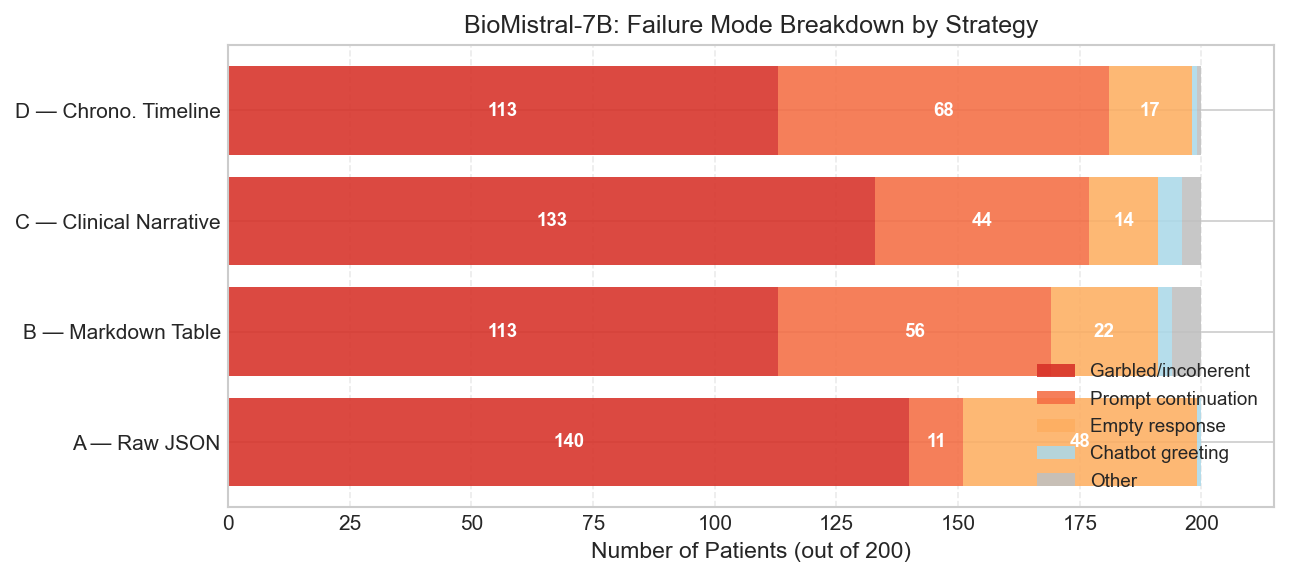
\includegraphics[width=\columnwidth]{figures/10_biomistral_failure_modes.png}
  \caption{BioMistral-7B failure mode breakdown by strategy (200 patients each).
           Garbled or incoherent output dominates across all four strategies. Prompt
           repetition (the model echoes the system prompt instead of responding)
           accounts for 11--68 patients per strategy. No strategy produces a
           parseable JSON response.}
  \label{fig:bio_failures}
\end{figure}

Figure~\ref{fig:f1_dist} shows the F1 distribution per model on each model's best
strategy. BioMistral's distribution is a degenerate spike at zero.

\begin{figure}[t]
  \centering
  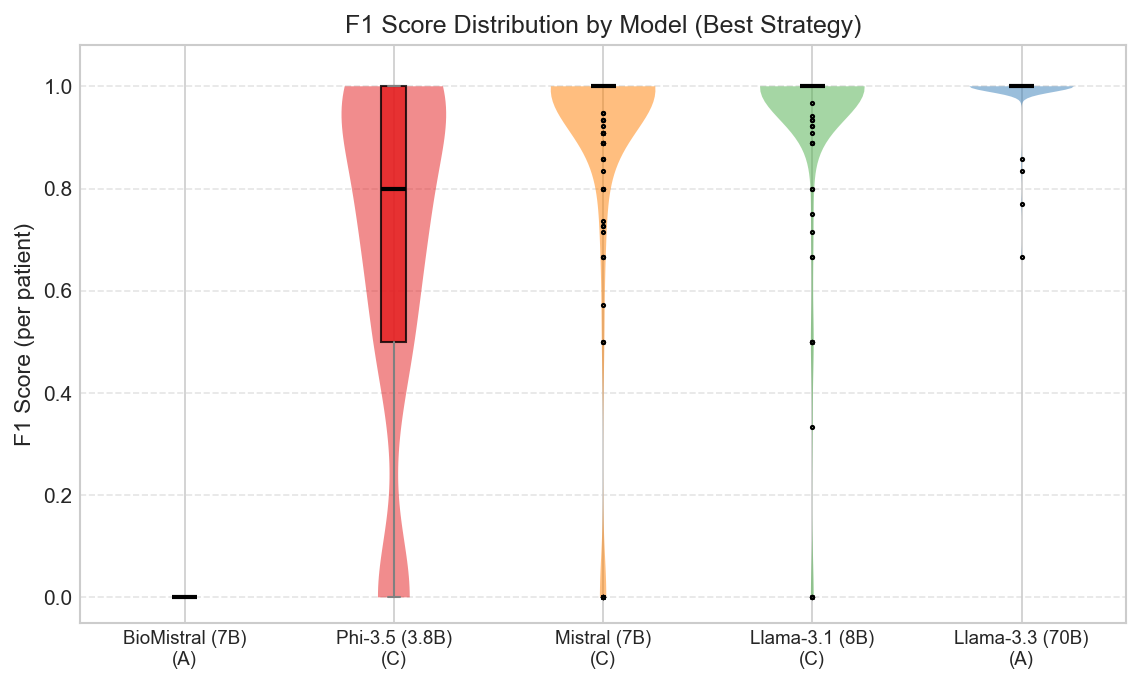
\includegraphics[width=\columnwidth]{figures/07_f1_distribution.png}
  \caption{F1 distribution per model on best strategy. BioMistral (all strategies)
           produces only zero-F1 outputs. Llama-3.3-70B has the tightest distribution
           near 1.0.}
  \label{fig:f1_dist}
\end{figure}
